\section{Kalibracja}
Po pomyślnym zestawieniu warstwy fizycznej posiadamy zdefiniowany wszystkie charakterystyki połączenia, 
które pozwolą w jednoznaczny sposób porozumieć sie z urządzeniem oraz żądać odpowiedzi na wysłaną wiadomość.
Kolejne komendy są już żądaniami wysokoziomowymi, które definiują użyteczne dla klienta polecenia służąca do zarządzania RET-em.
Jest ich znacznie więcej, aczkolwiek obranym celem pracy inżynierskiej było pomyślne przeprowadzenie kalibracji urządzenia, 
co pozwala w dalszym etapie ustawić zadany kąt odchylenia głównej wiązki sygnału z anteny.
W związku z tym, że oczekiwanie kalibracji przesłano przy pomocy ramki informacyjnej, bajt kontrolny posiada
charakterystyczną metodę jego ewaluacji przedstawioną wcześniej. Diagram sekwencji
potwierdza to, gdyż wiadomość odebrana przez urządzenie nadrzędne posiada wartość równą 0x30.
Ramka odebrana, na wyznaczenie liczby bajtów budujących odpowiedź posiada zarezerowane dwa bajty. 
Ciekawą obserwacją jest to, że odpowiedź równą 0x00 czyli OK można by zapisać przy pomocy jedynie jednego bajta, lecz optymalizacja
pamięci nie jest tutaj zastosowana.
\newline\newline
Z racji tego, że wiadomości tej warstwy korzystają z ramki informacyjnej, inną rolę pełni bajt kontrolny. Poza stałymi wartości bitów w bajcie 
każdorazowe wysłanie i odebranie wiadomości zmienia wartość sekcji P/F wcześniej wspomnianej. 
Dzięki temu można w łatwy sposób identyfikować czy wiadomość, którą otrzymujemy jest ta której oczekiwaliśmy. 
W związku z tym dla pierwszej wiadomości wysłanej przez urządzenie nadrzędne poprawną wartością będzie 0x10.
\newline
Kolejnym bajtem jest kod procedury, który ma wartość 0x31, co oznacza, że oczekujemy kalibracji urządzenia będącego zwykłym pojedynczym RET-em.
\newline
Z racji tego, że podczas tej komendy nie jest przesyłana żadna wartość dla tej procedury, dwa bajty zaalokowane dla długości parametru mają wartość \{0x00, 0x00\}
\begin{figure}[h!]
    \centering
    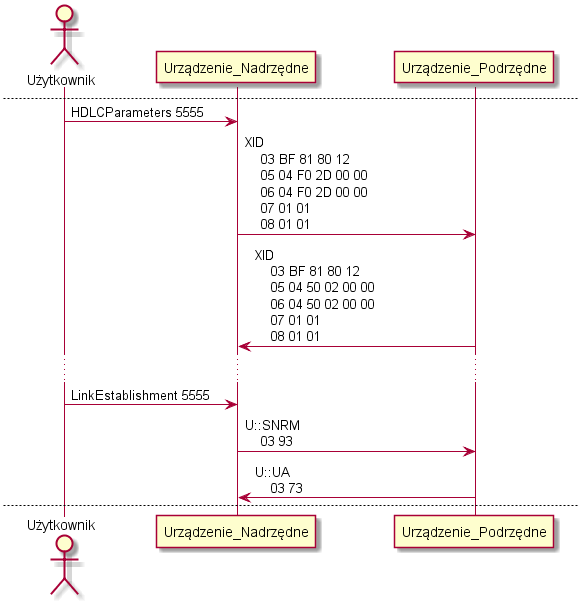
\includegraphics[scale=0.75]{out/Diagramy/UML_DiagramOfSequence_New/UML_DiagramOfSequence_New-page3.png}
    \caption{Negocjacja rozmiaru okna oraz payloadu ramki informacyjnej oraz ustanowienie normalnego trybu komunikacji.
        \newline(Opracowanie własne)}
    \label{fig:DiagramSequence_HDLCParameters_SNRM}
\end{figure}
\begin{figure}[h!]
    \centering
    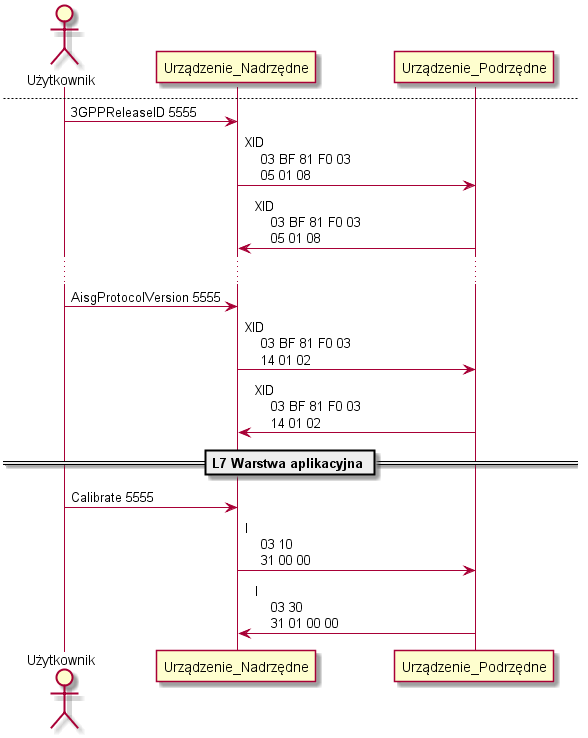
\includegraphics[scale=0.75]{out/Diagramy/UML_DiagramOfSequence_New/UML_DiagramOfSequence_New-page4.png}
    \caption{Negocjacja pozostałych parametrów HDLC oraz żadanie kalibracji urządzenia.
    \newline(Opracowanie własne)}
    \label{fig:DiagramSequence_3GPP_AISGVersion_Calibrate}
\end{figure}
